% Section content template for individual Educative lessons
% This file contains the actual content for a specific section
% Generated from Educative API section content

% Section: Class diagram for the Restaurant Management System
% Section ID: 6210405828657152
% Section Slug: class-diagram-for-the-restaurant-management-system
% Generated: 2025-12-14T12:23:58.301581

We'll create the class diagram for the restaurant management system. In the class diagram, we will first design the classes and then identify the relationships between classes according to the requirements of the restaurant management system design problem.

\subsection{Components of the restaurant management system}\label{x2gvpXM5TEQclmxCp4Kmk}
\\
As mentioned, we'll follow the bottom-up approach to design a class diagram for the restaurant management system.

\subsubsection{Person}\label{tl_jVASzwcMyEHTlgw6Gf}
\\
The \texttt{Person} class is extended by the \texttt{Waiter}, \texttt{Receptionist}, \texttt{Manager}, and \texttt{Customer} classes and stores the person's name, email, and phone number.

\begin{itemize}
\item
\protect\phantomsection\label{JH7eQSvzrdg0j4ES2K7To}
\texttt{Waiter}: Takes an order from the customer and generates the bill.
\item
\protect\phantomsection\label{yjZOeRa6Axk0Sg-O9pkug}
\texttt{Receptionist}: Creates a reservation.
\item
\protect\phantomsection\label{YhGtluYZaNAtLdzh99u5j}
\texttt{Manager}: Can update the seating plan and can also update the menu.
\item
\protect\phantomsection\label{ZASADCjSX_R_oNQg4umCJ}
\texttt{Customer}: This derived class can make reservations, place orders, and pay bills.
\end{itemize}

\begin{figure}[htbp]
 \centering
 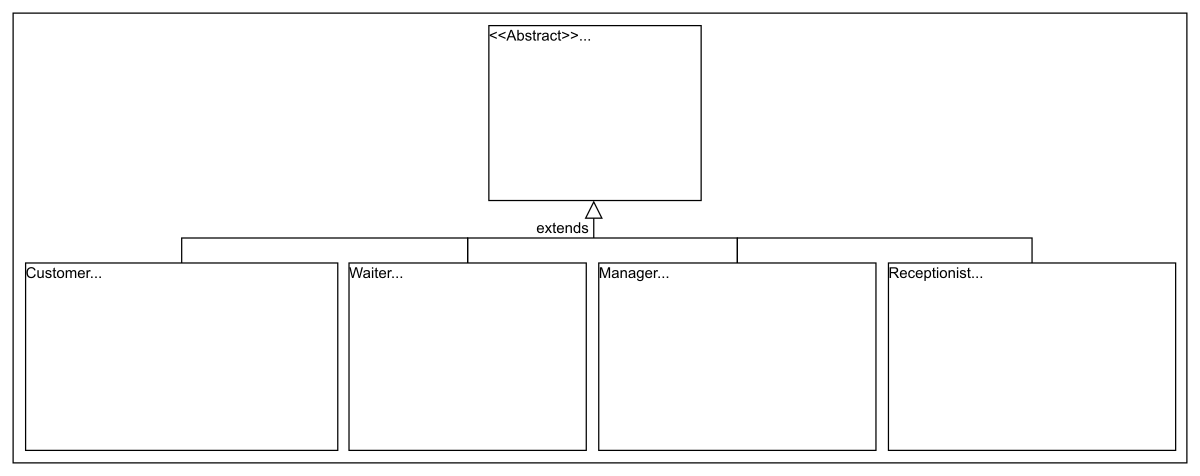
\includegraphics[width=0.5\textwidth]{Images/chapter_21/section_6210405828657152/4646960681058304.png}
 \caption{Person and its derived classes}
\end{figure}

\textbf{R3:} The server should be able to create an order for a table, add items for each person seated, and update the order as needed.
\\
\textbf{R6:} The system should allow for the reservation of tables.
\\
\textbf{R7:} The receptionist should be able to search for available tables by date and time and make a reservation.

\subsubsection{Table and table seat}\label{wB3tMNqvO5JPdMu8asGjF}
\\
The \texttt{Table} class is identified by an ID, a limited seating capacity, a specific location, and a status. A table may have multiple seats.

\begin{figure}[htbp]
 \centering
 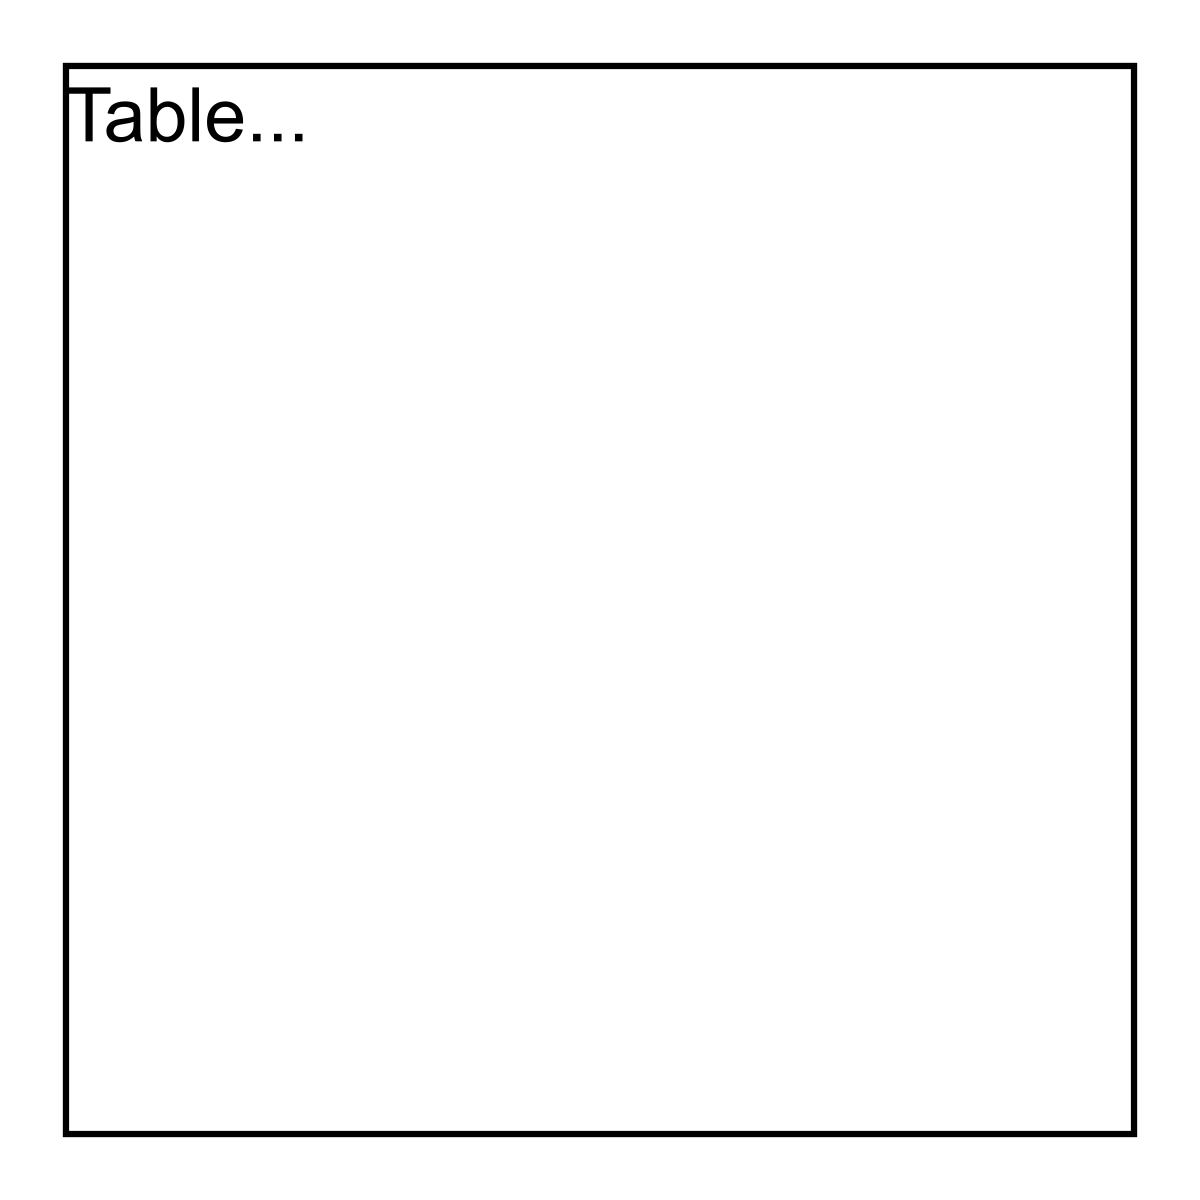
\includegraphics[width=0.5\textwidth]{Images/chapter_21/section_6210405828657152/5036505599705088.png}
 \caption{The Table class}
\end{figure}

\textbf{R5:} The system should be able to provide information about tables currently available for walk-in customers.
\\
\textbf{R6:} The system should allow for the reservation of tables.

\subsubsection{Meal and meal item}\label{q9vA_LupXO68l393G2SOb}
\\
The \texttt{Meal} class represents a customer's meal at a specific seat and table and contains a list of ordered items.
\\
\texttt{MealItem}: It is identified by a meal item ID and has a specific quantity that can be updated.

\begin{figure}[htbp]
 \centering
 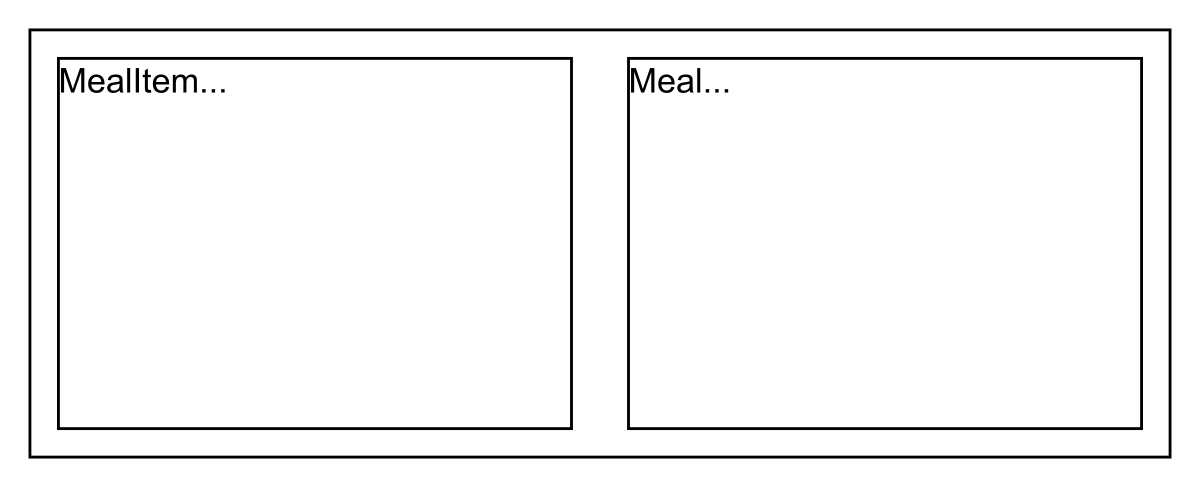
\includegraphics[width=0.5\textwidth]{Images/chapter_21/section_6210405828657152/6213821835116544.png}
 \caption{The Meal and MealItem classes}
\end{figure}

\textbf{R4:} Each person's order can consist of multiple items, each corresponding to a menu item.

\subsubsection{Menu, menu section, and menu item}\label{r1RCPcc6E3bPp_EjuOzE-}
\\
\texttt{Menu}\textbf{:} It has a unique ID, title, and description, and may have several sections.
\\
\texttt{MenuSection}\textbf{:} This class represents a menu section with an ID, a title, and a description. It may have multiple menu items.
\\
\texttt{MenuItem}\textbf{:} It is identified by an ID and has a title, description, and price that can be updated.

\begin{figure}[htbp]
 \centering
 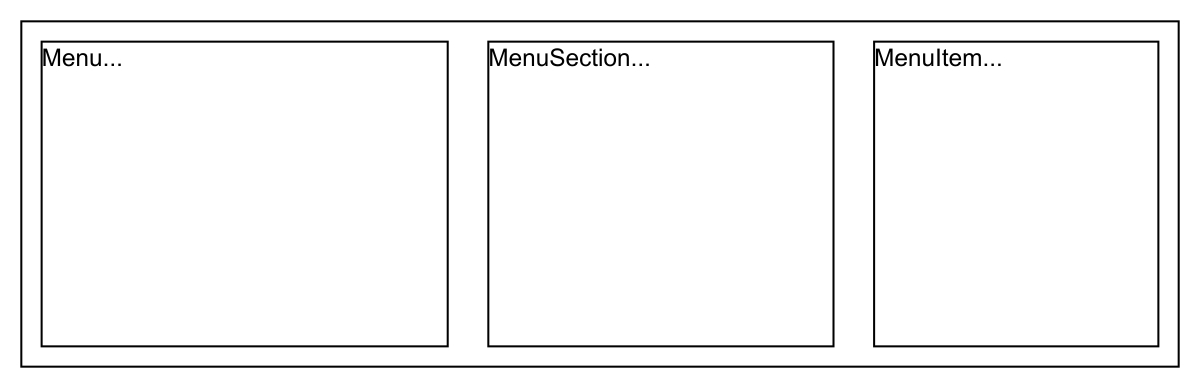
\includegraphics[width=0.5\textwidth]{Images/chapter_21/section_6210405828657152/6400627503398912.png}
 \caption{The Menu, MenuSection, and MenuItem classes}
\end{figure}

\textbf{R2:} Each branch will offer a menu with various sections and items.

\subsubsection{Order}\label{rvS13_EunZ2UFKtQ2er2l}
\\
The \texttt{Order} class is identified by an ID and has a status that can be updated regarding adding or removing meals.

\begin{figure}[htbp]
 \centering
 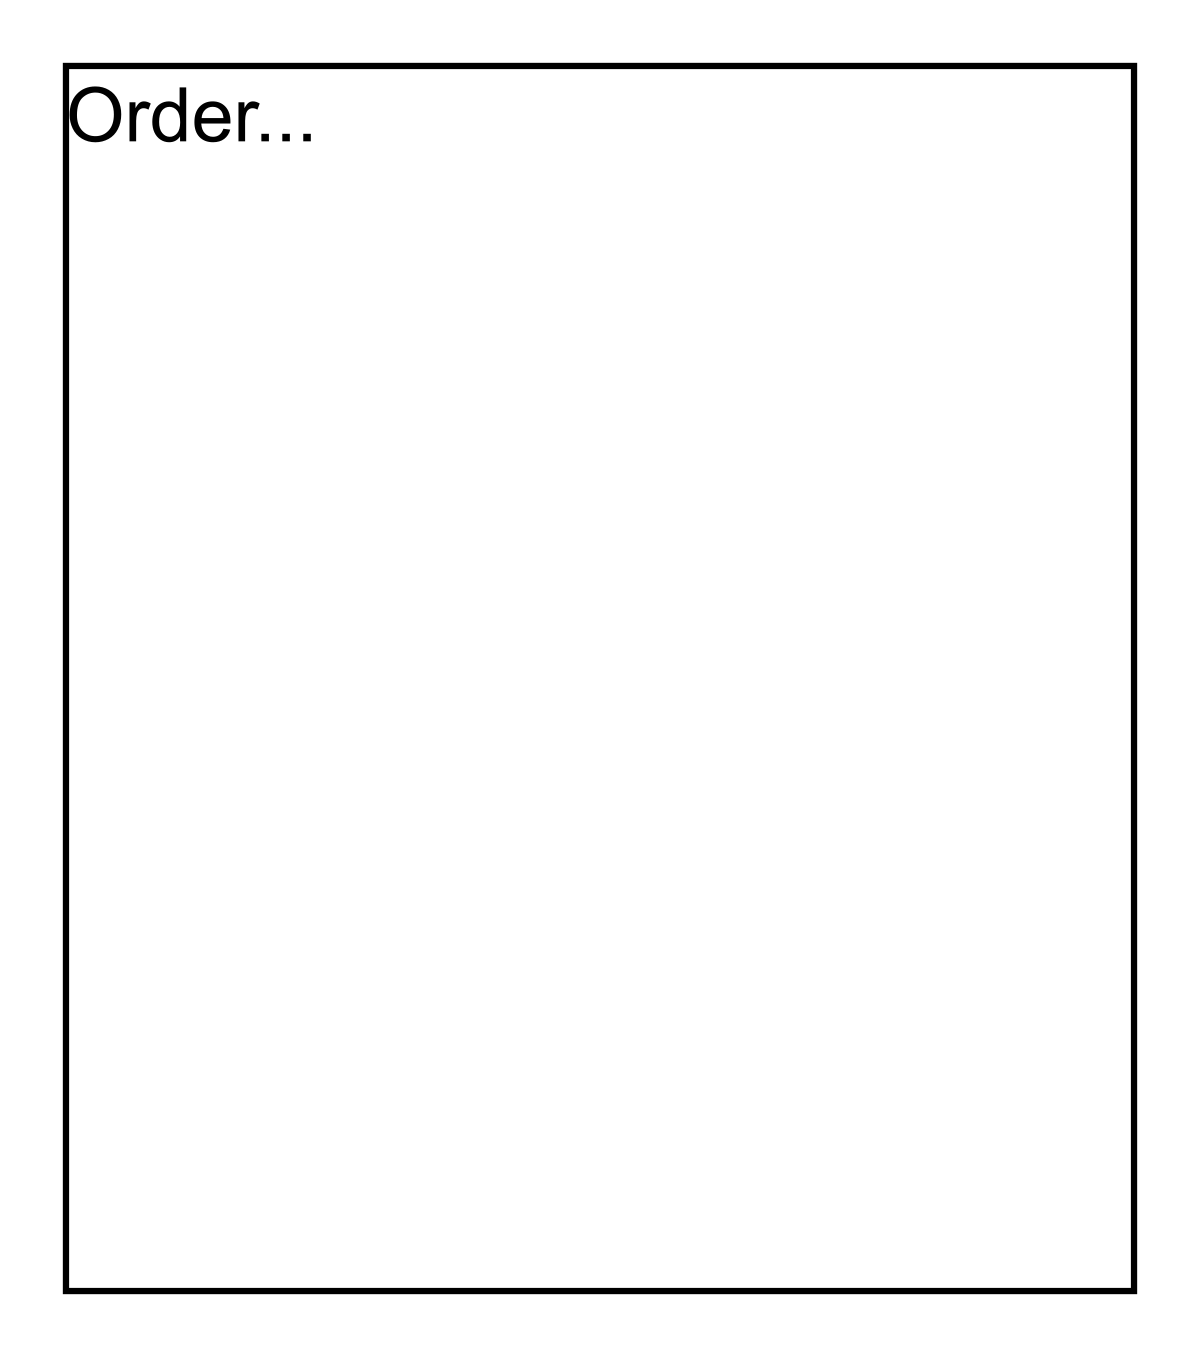
\includegraphics[width=0.5\textwidth]{Images/chapter_21/section_6210405828657152/6328108742213632.png}
 \caption{The Order class}
\end{figure}

\textbf{R3:} The server should be able to create an order for a table and add items for each person seated.
\\
\textbf{R4:} Each person's order can consist of multiple items, each corresponding to a menu item.

\subsubsection{Reservation}\label{KHwdcvWErS9cFyZy_orKS}
\\
A \texttt{Reservation} is made by the receptionist for the customer. This class has a reservation ID, reservation time, count, customer information, status, notes, and check-in time.

\begin{figure}[htbp]
 \centering
 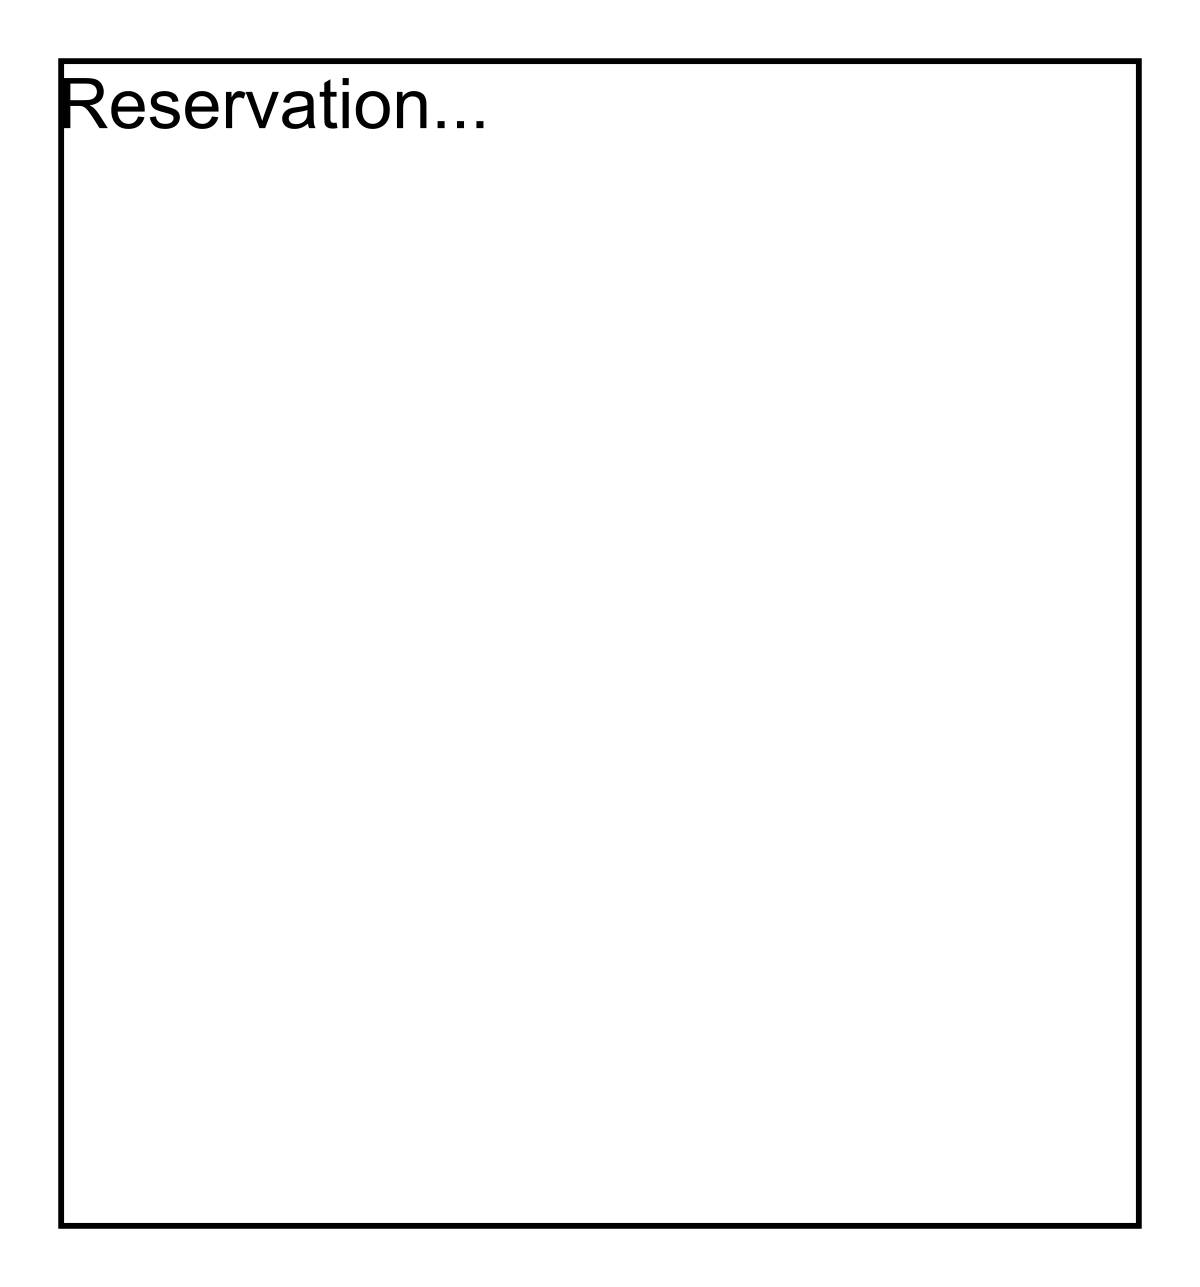
\includegraphics[width=0.5\textwidth]{Images/chapter_21/section_6210405828657152/5581664615792640.png}
 \caption{The Reservation class}
\end{figure}

\textbf{R6:} The system should allow for the reservation of tables.
\\
\textbf{R8:} The system should allow customers to make and cancel reservations.
\\
\textbf{R9:} The system should send notifications as the reservation time approaches.

\subsubsection{Payment}\label{LCOHL9ySKIAW-r--T0GX0}
\\
\texttt{Payment} is an abstract class extended by \texttt{CreditCardPayment} and \texttt{CashTransaction} as its child classes. This class stores a payment ID, the total amount, and the date.

\begin{itemize}
\item
\protect\phantomsection\label{hRZOTX_5hnDgQ_W2ybhC-}
\texttt{CreditCardPayment}: This derived class represents a credit card transaction.
\item
\protect\phantomsection\label{bCSAmXkXsP0HEi8WAa2US}
\texttt{CashTransaction}: This derived class represents a payment made in cash.
\end{itemize}

\begin{figure}[htbp]
 \centering
 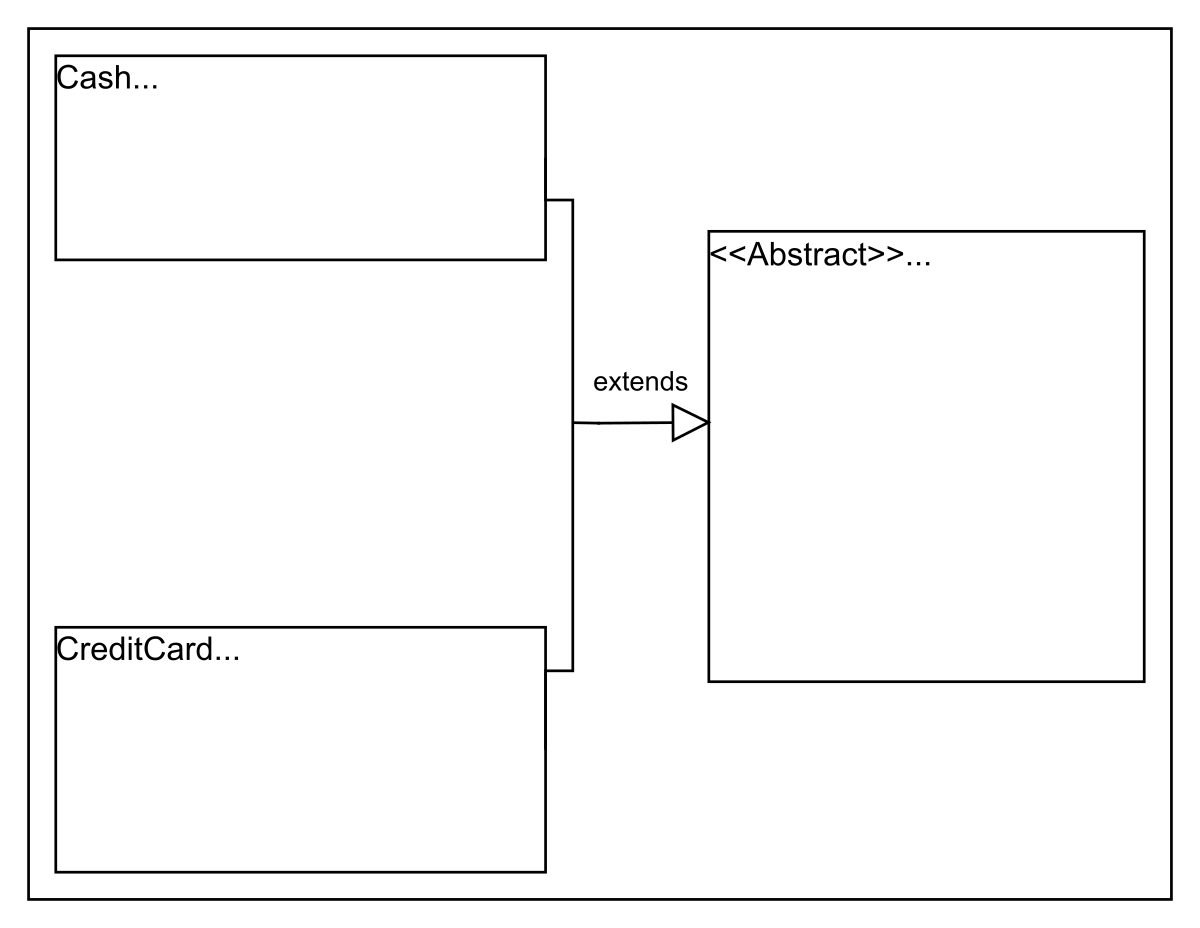
\includegraphics[width=0.5\textwidth]{Images/chapter_21/section_6210405828657152/5127121931206656.png}
 \caption{Payment and its derived classes}
\end{figure}

\textbf{R10:} Customers should be able to pay their bills with credit cards, checks, or cash.

\subsubsection{Bill}\label{akm59RignwGjQs0AU4-Es}
\\
The \texttt{Bill} class represents the total amount a customer has to pay based on the items ordered from the menu. This class stores an ID, the total amount to be paid, and the tax. Moreover, it records whether or not the bill was paid.

\begin{figure}[htbp]
 \centering
 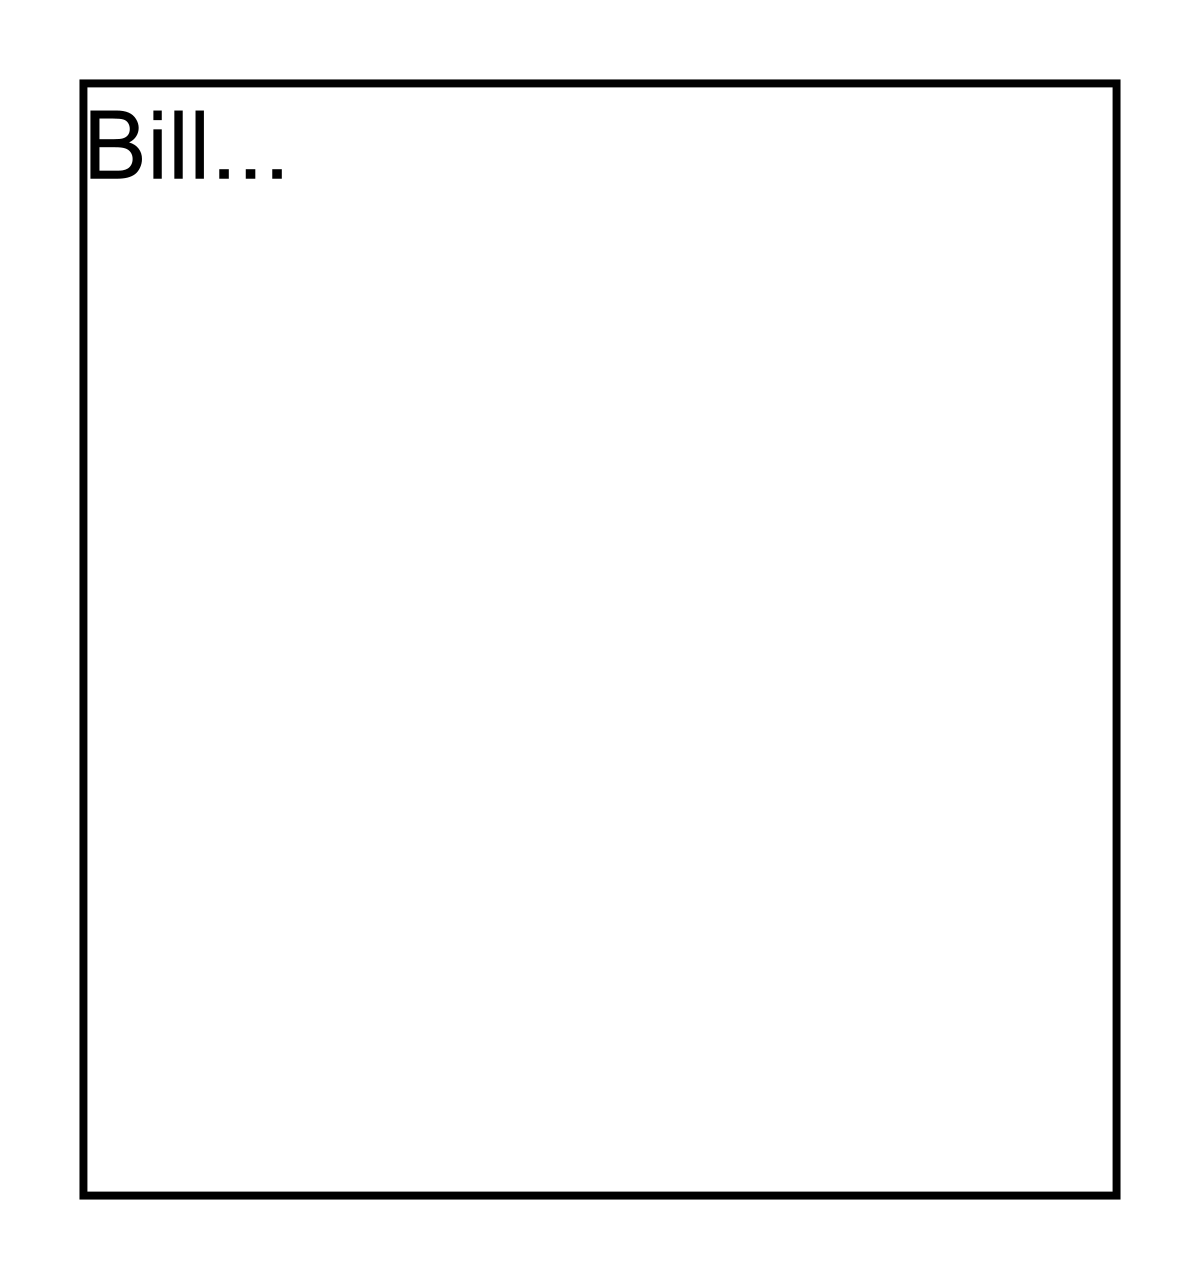
\includegraphics[width=0.5\textwidth]{Images/chapter_21/section_6210405828657152/4831124818624512.png}
 \caption{The Bill class}
\end{figure}

\textbf{R10:} Customers should be able to pay their bills with credit cards, checks, or cash.

\subsubsection{Notification}\label{wWUdn8OACHbE_do-ONY35}
\\
A \texttt{Notification} is a message sent to a customer from the restaurant. Every
\texttt{Notification} has a specific ID, the date it was sent, and the content the customer wrote.

\begin{figure}[htbp]
 \centering
 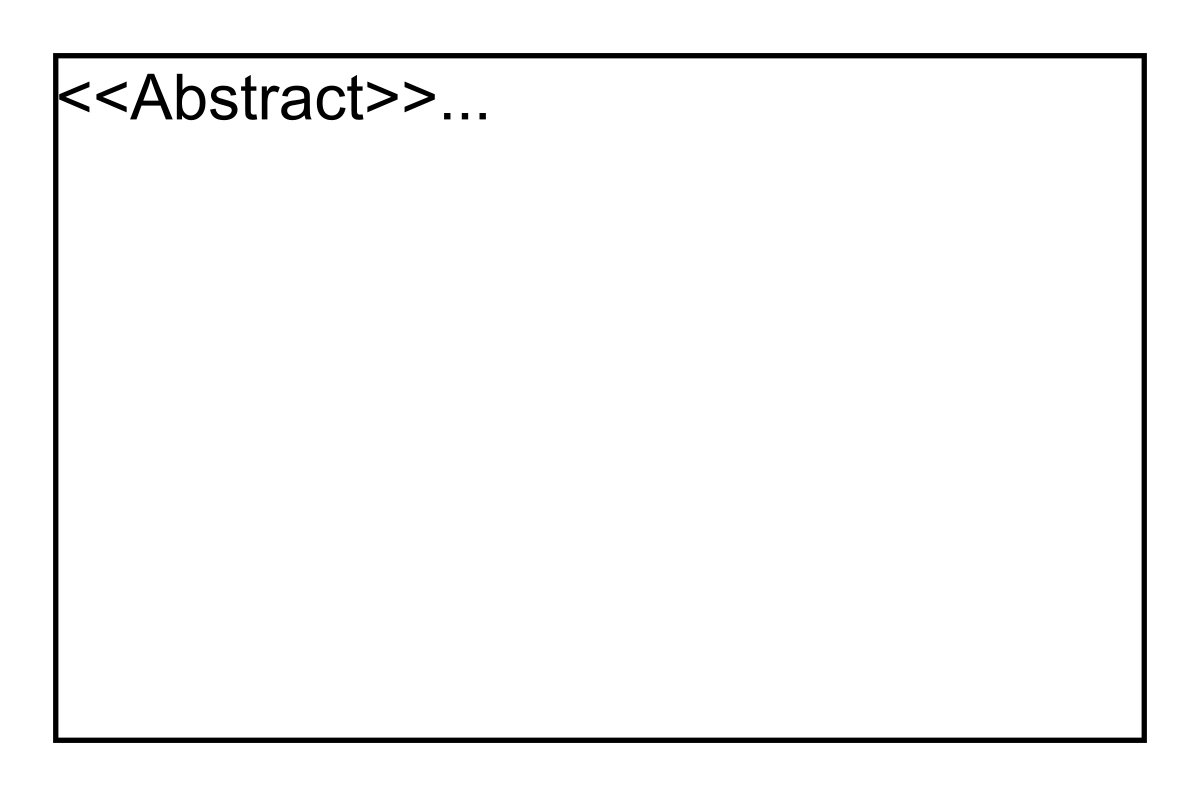
\includegraphics[width=0.5\textwidth]{Images/chapter_21/section_6210405828657152/5063133549690880.png}
 \caption{The Notification and its derived classes}
\end{figure}

\textbf{R9:} The system should send notifications as the reservation time approaches.

\subsubsection{Seating chart and branch}\label{scNxjp7yNL_sm1kpWZdLo}
\\
\texttt{TableConfiguration}\textbf{:} This class represents the seating plan of a restaurant. A unique ID identifies it.
\\
\texttt{Branch}\textbf{:} This class represents the branches of a restaurant. Every \texttt{Branch} has a specific name and location.

\begin{figure}[htbp]
 \centering
 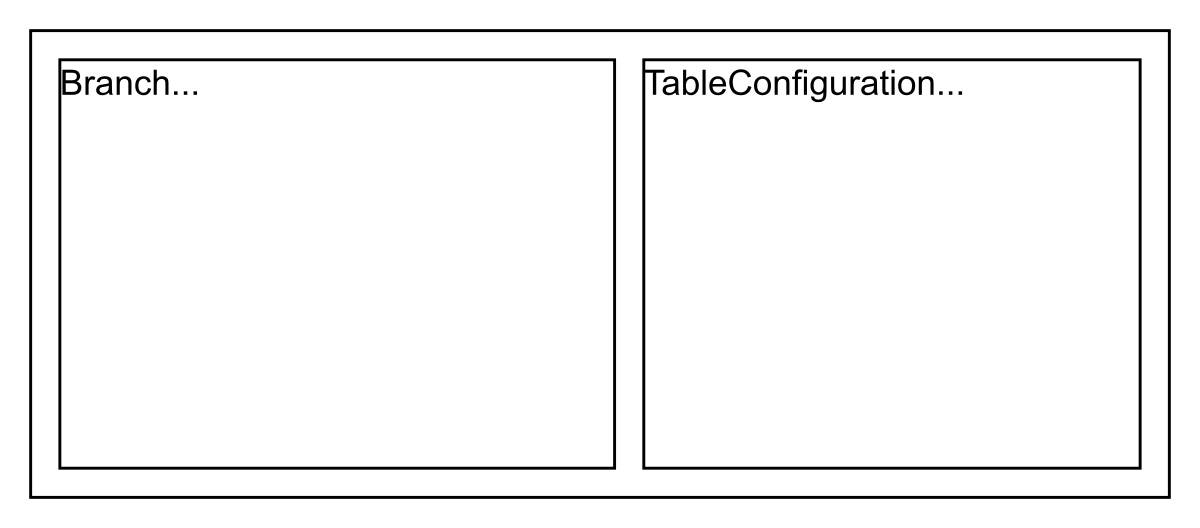
\includegraphics[width=0.5\textwidth]{Images/chapter_21/section_6210405828657152/6205681571856384.png}
 \caption{The SeatingChart, Branch, and Restaurant classes}
\end{figure}

\textbf{R1:} The restaurant can have multiple branches.
\\
\textbf{R2:} Each branch will offer a menu with various sections and items.
\\
\textbf{R11:} Each branch may have different configurations of tables.

\subsubsection{Enumerations and custom data types}\label{4YJM0lM0YV79ESfOz2TDC}
\\
\texttt{TableStatus}\textbf{:} This enumeration checks whether a table is reserved, occupied, or free.
\\
\texttt{OrderStatus}\textbf{:} This enumeration keeps track of a customer's order status.
\\
\texttt{PaymentStatus}\textbf{:} This enumeration keeps track of an order's payment status by the customer.
\\
\texttt{ReservationStatus}\textbf{:} This enumeration represents the reservation status of a table for a customer.

\begin{figure}[htbp]
 \centering
 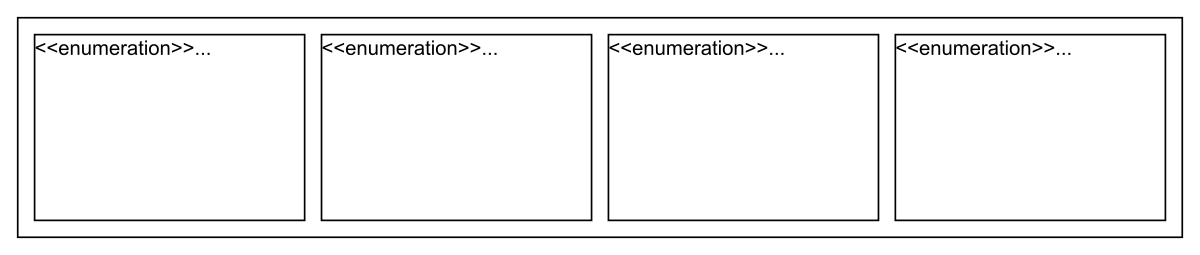
\includegraphics[width=0.5\textwidth]{Images/chapter_21/section_6210405828657152/4896180897972224.png}
 \caption{Enums in the restaurant management system}
\end{figure}

\texttt{Address}: This custom data type represents the address of the restaurant's branch or a person.

\begin{figure}[htbp]
 \centering
 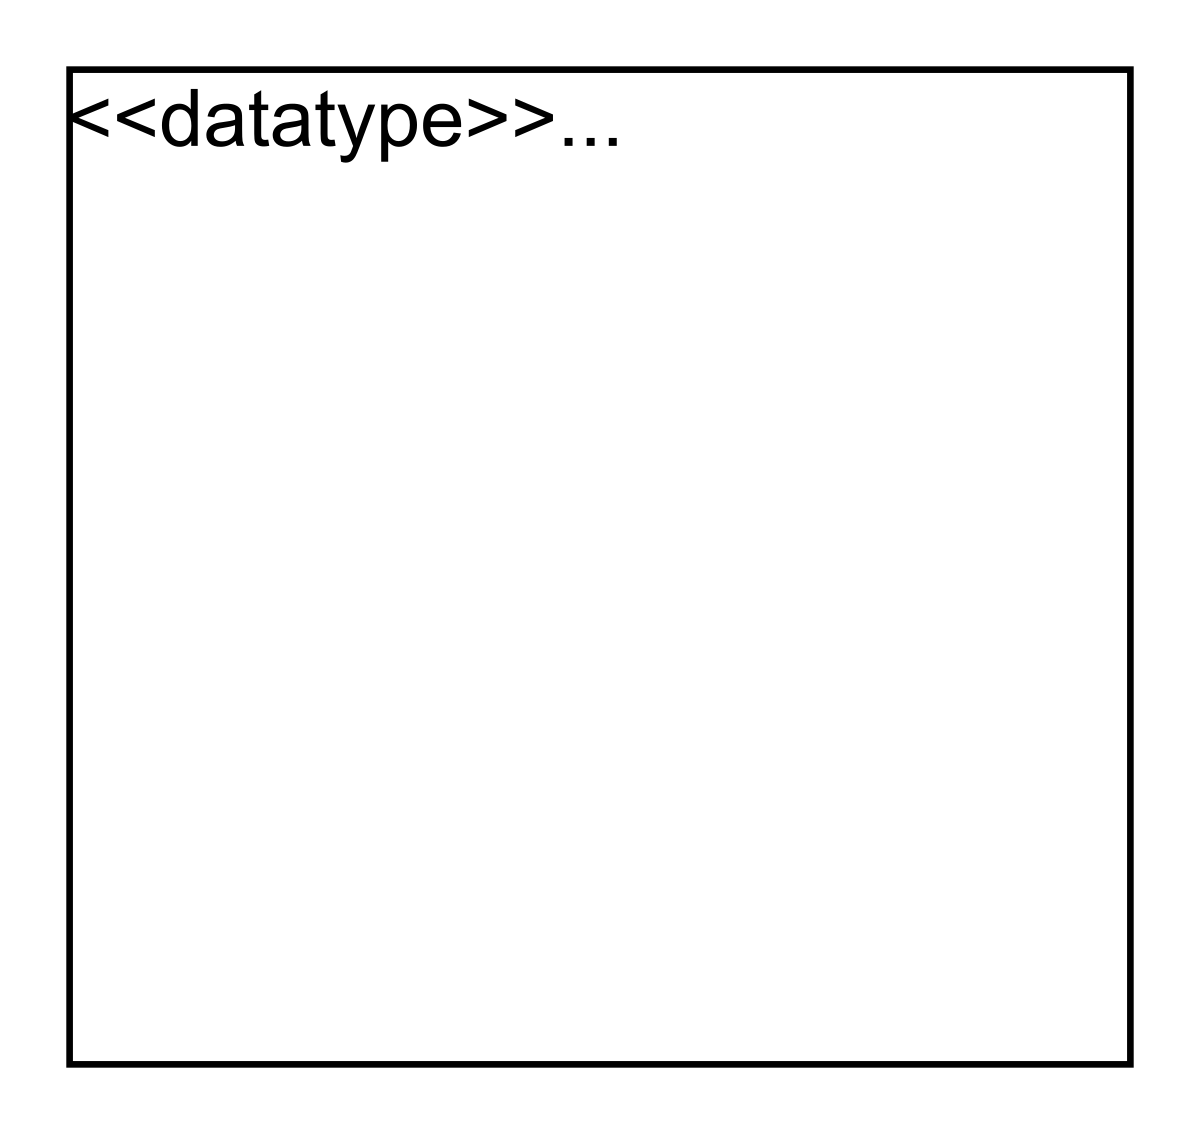
\includegraphics[width=0.5\textwidth]{Images/chapter_21/section_6210405828657152/5152497659150336.png}
 \caption{Class diagram of the Address custom data type}
\end{figure}

\subsection{Relationship between the classes}\label{sTaz_5hm5Nq6h9Myj6-A7}
\\
Now, we'll discuss the relationships between the classes we have defined above in our restaurant management system.

\subsubsection{Association}\label{WKCob0gqnfJ88O7i89QAE}
\\
The class diagram has the following association relationships:
\\
\paragraph{One-way Association}\label{c-r91Cjdmrn_SCtlJkgeQ}

\begin{itemize}
\item
\protect\phantomsection\label{Jbclan5YVlhHtu25X_nbG}
The \texttt{Waiter}, \texttt{Manager}, and \texttt{Receptionist} class has a one-way association with the \texttt{Branch}.
\item
\protect\phantomsection\label{ImG41TXTBl6W-YOtnJfPV}
The \texttt{MealItem} class has a one-way association with \texttt{MenuItem}.
\item
\protect\phantomsection\label{P3JRJrehxOOG_TFW6EApK}
The \texttt{Waiter} class has a one-way association with \texttt{Order}.
\item
\protect\phantomsection\label{fO723HusQateJxEGz8HX2}
The \texttt{Order} class has a one-way association with \texttt{Table}.
\item
\protect\phantomsection\label{_dysmbkccSVrJWwe4gFX9}
The \texttt{Receptionist} class has a one-way association with \texttt{Reservation}.
\item
\protect\phantomsection\label{R5KzL0iWgcEE_RwgTWbEK}
The \texttt{Reservation} class has a one-way association with \texttt{Table}.
\end{itemize}

\begin{figure}[htbp]
 \centering
 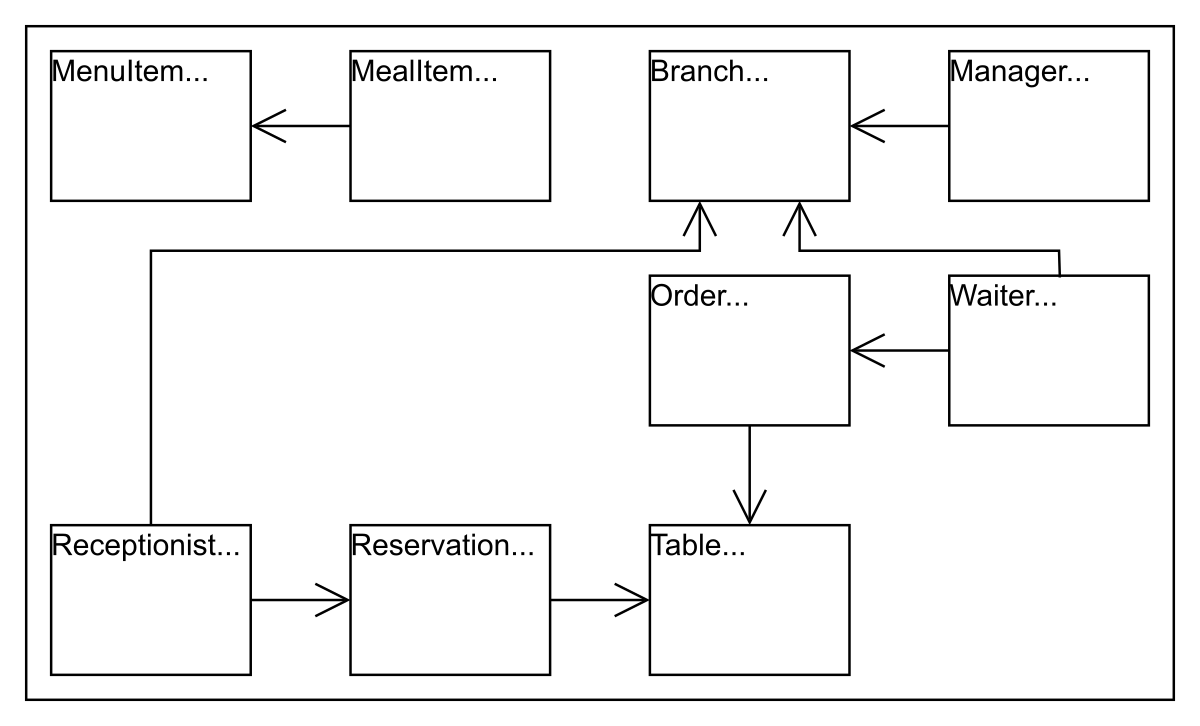
\includegraphics[width=0.5\textwidth]{Images/chapter_21/section_6210405828657152/5266985595043840.png}
 \caption{The one-way association relationship between classes}
\end{figure}

\paragraph{Two-way Association}\label{ScyajZPcdAbVHGc4-lL41}

\begin{itemize}
\item
\protect\phantomsection\label{1pNWOgODhIZ493uB7OeCr}
The \texttt{Branch} and \texttt{Menu} classes are associated with each other.
\item
\protect\phantomsection\label{AIKExE4snoTPtyu1_bye8}
The \texttt{Customer} and \texttt{Reservation} classes are associated with each other.
\item
\protect\phantomsection\label{tgFJvSIdjX8KNeI2zJhTa}
The \texttt{Reservation} and \texttt{Notification} classes are associated with each other.
\item
\protect\phantomsection\label{KPU3zM8mUI0KnTkQxYBr_}
The \texttt{Payment} and \texttt{Bill} classes are associated with each other.
\item
\protect\phantomsection\label{daCbRX_b8XNWQ8e0a_DZb}
The \texttt{Bill} and \texttt{Order} classes are associated with each other.
\end{itemize}

\begin{figure}[htbp]
 \centering
 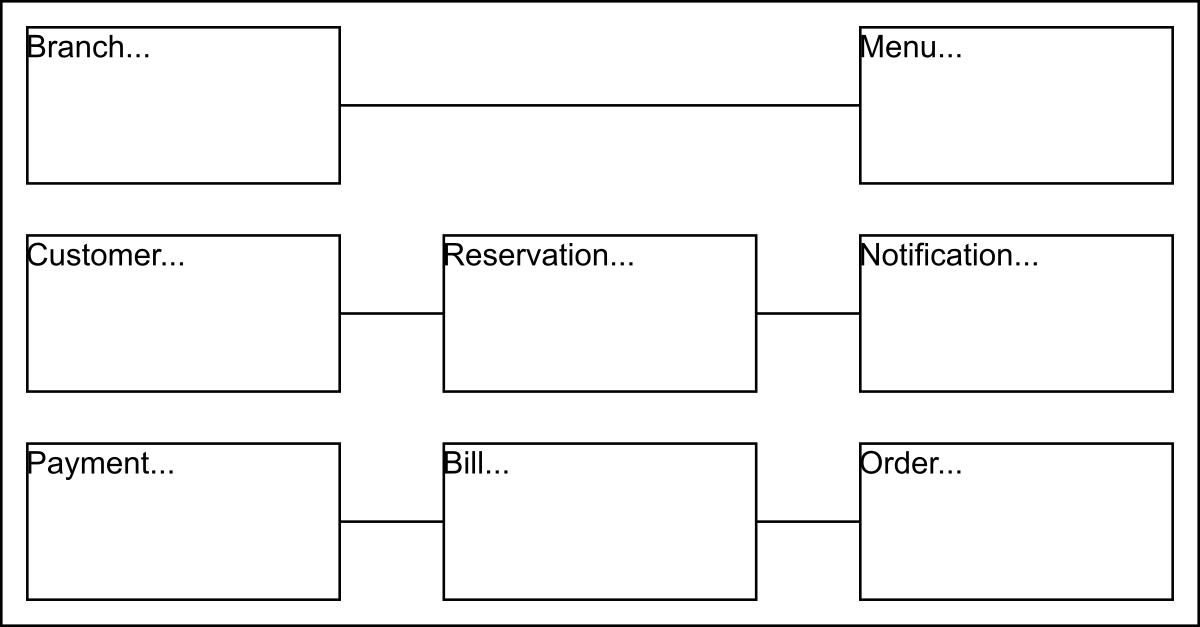
\includegraphics[width=0.5\textwidth]{Images/chapter_21/section_6210405828657152/5625009889607680.png}
 \caption{The two-way association relationship between classes}
\end{figure}

\subsubsection{Composition}\label{pKkshKviSb_tnohckOykm}
\\
The class diagram has the following composition relationships.

\begin{itemize}
\item
\protect\phantomsection\label{AN5AXDVe2xTidZiLuxmLU}
The \texttt{Branch} class is composed of \texttt{TableConfiguration}.
\item
\protect\phantomsection\label{4YoDlCsyYWftYniYpUTCs}
The \texttt{Meal} class is composed of \texttt{MealItem} and \texttt{Table}.
\item
\protect\phantomsection\label{4fYqEXvh1ybS0_ReBxhFz}
The \texttt{Order} class is composed of \texttt{Meal}.
\item
\protect\phantomsection\label{m4Wt5wbV94sLrmliyf8Rr}
The \texttt{MenuSection} class is composed of \texttt{MenuItem}.
\item
\protect\phantomsection\label{ZSWljlowxR04AcZTa1ygI}
The \texttt{Menu} class is composed of \texttt{MenuSection}.
\end{itemize}

\begin{figure}[htbp]
 \centering
 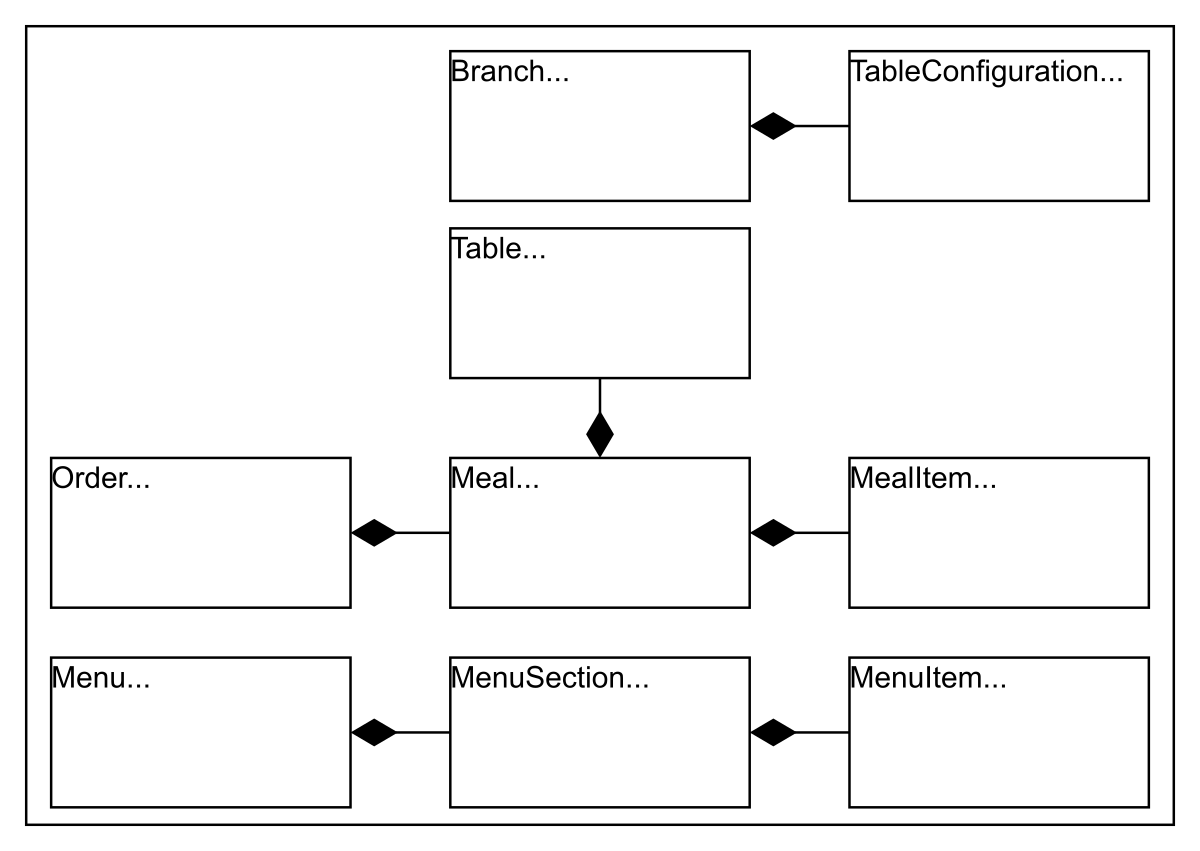
\includegraphics[width=0.5\textwidth]{Images/chapter_21/section_6210405828657152/6401858951053312.png}
 \caption{The composition relationship between classes}
\end{figure}

\subsubsection{Inheritance}\label{gQxKRQMQnoi-iM4O92Swb}
\\
The following classes show an inheritance relationship:

\begin{itemize}
\item
\protect\phantomsection\label{lIm1YbqOPAezRnyeVYv-v}
All the classes, \texttt{Manager}, \texttt{Waiter}, \texttt{Receptionist}, and \texttt{Customer}, extend the \texttt{Person} class.
\item
\protect\phantomsection\label{i4sIWHppI3rAQD1K2nj0g}
\texttt{Payment} class is extended by \texttt{CreditCardPayment} and \texttt{CashTransaction}.
\end{itemize}
\begin{quote}
\textbf{Note:} We have already discussed the inheritance relationship between classes in the component section above one by one.
\end{quote}
\subsection{Class diagram for the restaurant management system}\label{57zQtma_KlmAKjJvZkv6T}
\\
This section outlines the multiplicity (cardinality) relationships between the main classes in our restaurant management system. We explain the allowed number of instances on each side for each relationship and the real-world or design rationale behind the connection. Understanding these relationships is key to modeling how different entities interact and collaborate to support key workflows in the system.

\begin{table}[h!]
\centering
\begin{tabular}{|p{3.5cm}|p{3.5cm}|p{3cm}|p{6.5cm}|}
\hline
\textbf{Source} & \textbf{Target} & \textbf{Multiplicity} & \textbf{Reason} \\
\hline
Address & Customer & 1--1 & A customer has exactly one address. \\
\hline
Customer & Reservation & 1--0..* & A customer can make multiple reservations. \\
\hline
Customer & Order & 1--0..* & A customer can place multiple orders. \\
\hline
Reservation & Table & 0..*--1 & A reservation can be made for multiple tables. \\
\hline
Table & Branch & 1--1 & A table belongs to exactly one branch. \\
\hline
Branch & TableConfiguration & 1--0..* & A branch can have multiple table configurations. \\
\hline
TableConfiguration & Table & 1--0..* & A table configuration can relate to multiple tables. \\
\hline
Order & Table & 1--0..* & An order can be associated with multiple tables. \\
\hline
Order & Bill & 1--0..* & An order can generate multiple bills. \\
\hline
Bill & Payment & 1--1 & A bill can have one payment. \\
\hline
Bill & Cash & 1--0..1 & A bill can be paid in cash. \\
\hline
Bill & CreditCard & 1--0..1 & A bill can be paid via credit card. \\
\hline
Waiter & Order & 1--0..* & A waiter can handle multiple orders. \\
\hline
Waiter & Table & 1--0..* & A waiter can handle multiple tables. \\
\hline
Order & Meal & 1--0..* & An order can contain multiple meals. \\
\hline
Meal & MenuItem & 1--0..* & A meal can have multiple menu items. \\
\hline
MenuSection & MenuItem & 1--0..* & A menu section can contain multiple menu items. \\
\hline
Menu & MenuSection & 1--0..* & A menu can have multiple menu sections. \\
\hline
Menu & TableConfiguration & 1--0..* & A menu can be linked to multiple table configurations. \\
\hline
Manager & Branch & 1--0..* & A branch may have multiple managers. \\
\hline
Receptionist & Reservation & 1--0..* & A receptionist can manage multiple reservations. \\
\hline
Reservation & Notification & 0..*--1 & A reservation can have multiple notifications. \\
\hline
Waiter & Branch & 1--0..* & A branch may have multiple waiters. \\
\hline
Receptionist & Branch & 1--0..* & A branch may have multiple receptionists. \\
\hline
\end{tabular}
\caption{Entity Relationships and Multiplicities in a Restaurant Management System}
\label{tab:restaurant_entity_relationships}
\end{table}


Here's the complete class diagram for the restaurant management system:

\begin{figure}[htbp]
 \centering
 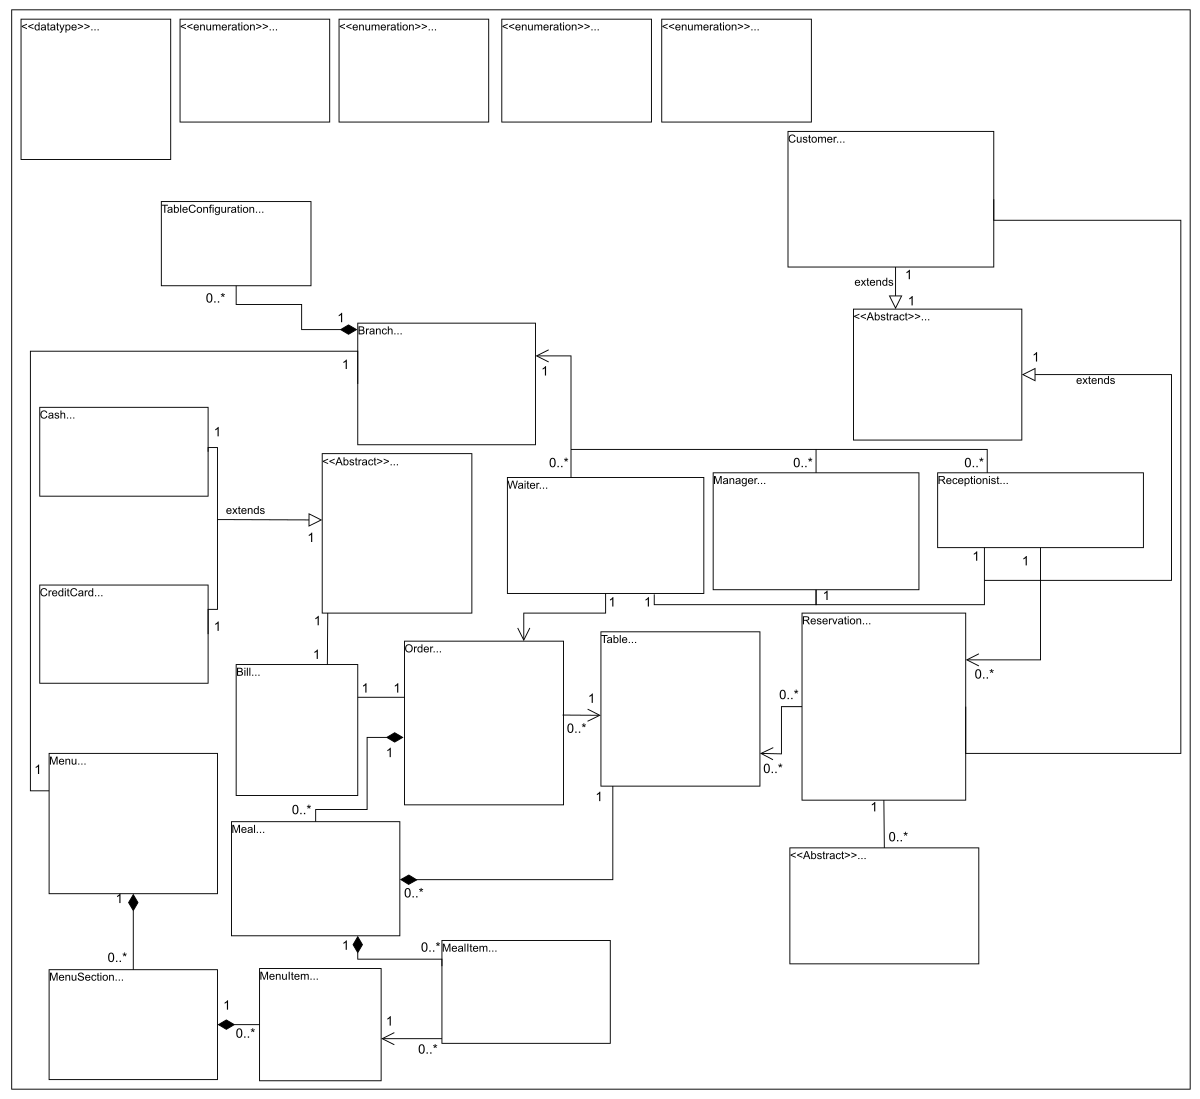
\includegraphics[width=0.5\textwidth]{Images/chapter_21/section_6210405828657152/5078437872926720.png}
 \caption{The class diagram of the restaurant management system}
\end{figure}

\subsection{Design pattern}\label{dJVhhtZ69C2EnAGmRBeW8}
\\
The following design patterns have been used in the class diagram:

\begin{itemize}
\item
\protect\phantomsection\label{NC12vemIGtIL6OnZc3u-A}
We know that a restaurant can accept different types of payments, such as cash or credit cards. To model this behavior, we can use the Strategy design pattern.
\item
\protect\phantomsection\label{vQr27mYtDrvE_w8hbII8q}
Every restaurant payment follows a general process: prepare the bill, initiate the transaction, and finalize payment. To model this behavior, we can use the Template Method design pattern.
\item
\protect\phantomsection\label{ScdmsWTxOJrsJvhXtvPty}
A restaurant menu is organized into sections (like starters, main courses, and desserts), containing multiple items. The Composite design pattern can be used to model this hierarchical structure.
\item
\protect\phantomsection\label{m7T12llhKex1JDLHkxFmm}
We know that employees and customers in a restaurant share some common attributes like name, email, and address, but have different roles and responsibilities. We can use inheritance and polymorphism to model this shared behavior with specialization.
\end{itemize}

\subsection{AI-powered trainer}\label{LmlccgYDisZzQQV_9C3SI}
\\
At this stage, everything should be clear. If you encounter any confusion or ambiguity, feel free to utilize the interactive AI-enabled widget below to seek clarification. This tool is designed to help you strengthen your understanding of the concepts.

\begin{figure}[htbp]
 \centering
 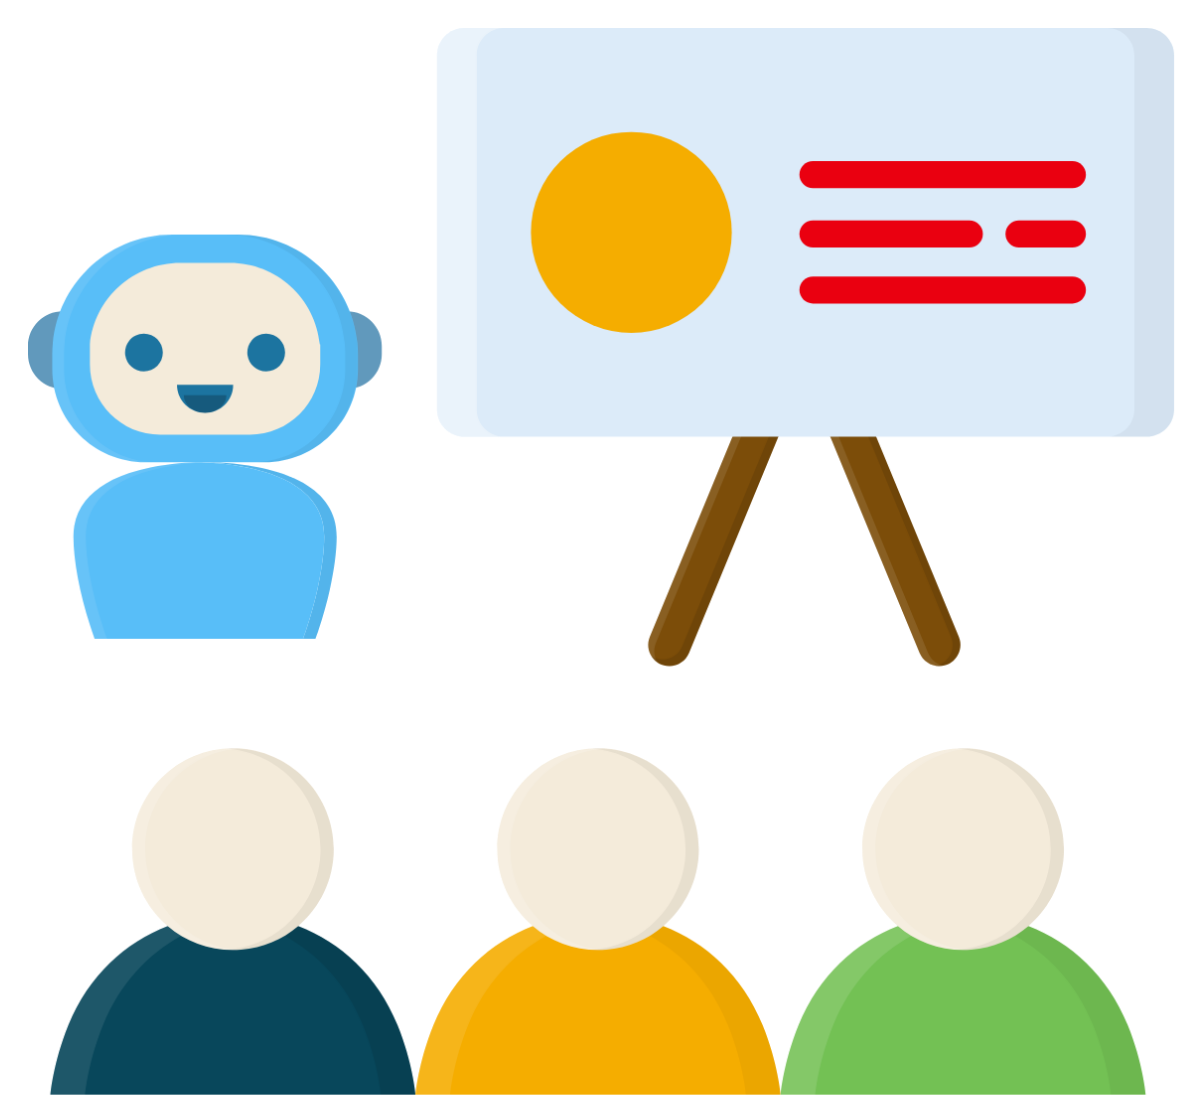
\includegraphics[width=0.15\textwidth]{Images/chapter_21/section_6210405828657152/6682962996101120.png}
 
\end{figure}

\subsection{Additional requirements}\label{kQH0KwogA5FkqNkrIul46}
\\
The interviewer can introduce some additional requirements in the given restaurant management system, or they can ask some follow-up questions. Let 's see examples of the additional requirements:
\\
\textbf{Discount:} A discount will be applied to the payment depending on special events such as the New Year, an anniversary, a branch opening, etc. The class diagram provided below shows the relationship of \texttt{Discount} with the \texttt{Payment} class:

\begin{figure}[htbp]
 \centering
 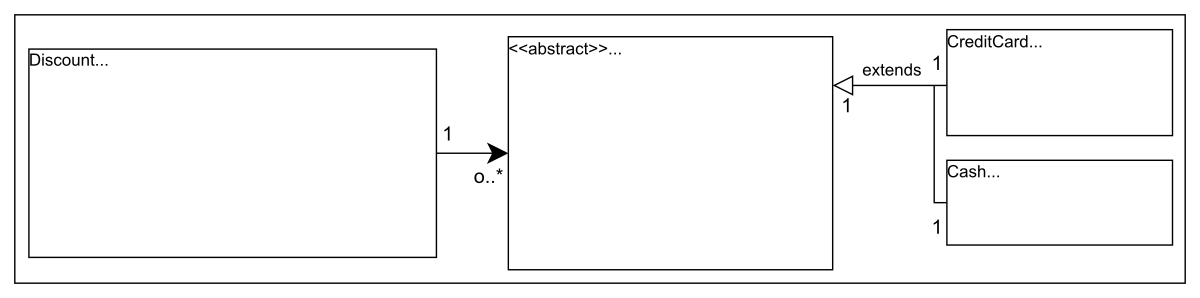
\includegraphics[width=0.5\textwidth]{Images/chapter_21/section_6210405828657152/6329932018745344.png}
 \caption{The relationship of the Discount class with the Payment class}
\end{figure}

We can update the \texttt{Payment} class to include an \texttt{applyDiscount()} method that can be invoked during the transaction process. This method would check if a discount is applicable based on the payment's creation date and, if so, apply the discount to the total amount.
\\
We have completed the class diagram of the restaurant management system according to the requirements. In the next lesson, let's design its sequence diagram.

% End of section content